\section{Long Short Term Memory}
\label{chap:Long Short Term Memory}

  %%%%%%%%%%%%%%%%%%%%%%%%%%%%
  % SUBSECTION               %
  %%%%%%%%%%%%%%%%%%%%%%%%%%%%
\subsection{Introduction}
As we know from the previous section that RNNs work just fine when we are dealing with short-term dependencies.
When we deal with long term dependencies problems like vanishing or exploding gradients appear.RNNs fail to understand the context behind an input, Something that was said long before, cannot be recalled when making predictions in the present.The relevant information may be separated from the point where it is needed, by a huge load of irrelevant data.\\
We know that for a conventional feed-forward neural network, the weight updating that is applied on a particular layer is a multiple of the learning rate, the error term from the previous layer and the input to that layer. Thus, the error term for a particular layer is somewhere a product of all previous layers’ errors. When dealing with activation functions like the sigmoid function, the small values of its derivatives (occurring in the error function) gets multiplied multiple times as we move towards the starting layers. As a result of this, the gradient almost vanishes as we move towards the starting layers, and it becomes difficult to train these layers, problem of Vanishing Gradients.\\
Also Exploding Gradients problem, happens when error gradients can accumulate during an update and results in very large gradients. These in turn result in large updates to the network weights, and in turn, an unstable network. At an extreme, the values of weights can become so large as to overflow and result in NaN values. The explosion occurs through exponential growth by repeatedly multiplying gradients through the network layers that have values larger than 1.0.\\
RNN remembers things for just small durations of time, i.e. if we need the information after a small time it may be reproducible, but once a lot of words are fed in, this information gets lost somewhere. This issue can be resolved by applying a slightly tweaked version of RNNs – the Long Short-Term Memory Networks.\cite{web005}

\subsection{Improvement over RNN: LSTM}
In order to add a new information, it transforms the existing information completely by applying a function. Because of this, the entire information is modified, on the whole, i.e. there is no consideration for ‘important’ information and ‘not so important’ information.\\
LSTMs on the other hand, make small modifications to the information by multiplications and additions. With LSTMs, the information flows through a mechanism known as cell states. This way, LSTMs can selectively remember or forget things. The information at a particular cell state has three different dependencies.\\
These dependencies can be generalized to any problem as:\\
\indent$\bullet$ The previous cell state (i.e. the information that was present in the memory after the previous time step)\\
\indent$\bullet$ The previous hidden state (i.e. this is the same as the output of the previous cell)\\
\indent$\bullet$ The input at the current time step (i.e. the new information that is being fed in at that moment)\\\\
 LSTMs, where they do not manipulate the entire information but rather modify them slightly, they are able to forget and remember things selectively. How do they do so ?, it is what we are going to learn.
 \subsection{Inside LSTM Cell}
 A typical LSTM network is comprised of different memory blocks called cells.
   There are two states that are being transferred to the next cell; the cell state and the hidden state.The memory blocks are responsible for remembering things and manipulations to this memory is done through three major mechanisms, called gates. Each of them is being discussed below.
 \begin{figure}[H]%
    \center%
    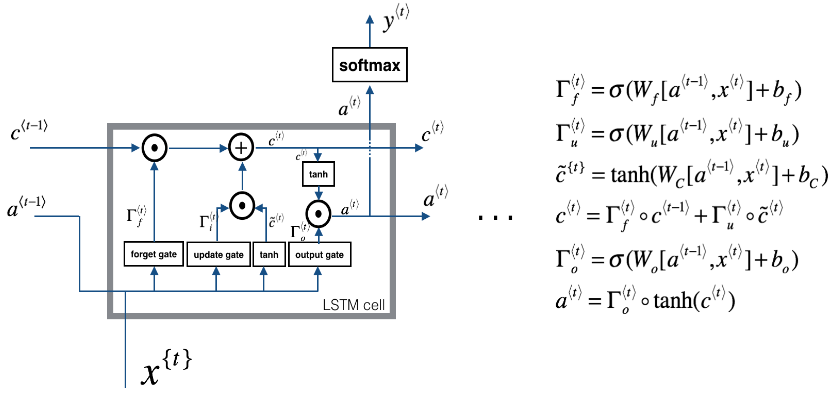
\includegraphics[width=\textwidth]{images/amir/cap1.png}%
     % you need to add the caption for the list of figures
    \caption[This is lstm-inside image]{a look inside LSTM cell}\label{fig:lstm inside}%
  \end{figure}
  \subsubsection{Forget Gate}
  A forget gate is responsible for removing information from the cell state.The information that is no longer required for the LSTM to understand things or the information that is of less importance is removed via multiplication of a filter. This is required for optimizing the performance of the LSTM network.\\
  This gate takes in two inputs; $x^t$ input at that particular time step and $a^{(t-1)}$ hidden state from the previous cell or the output of the previous cell. The given inputs are multiplied by the weight matrices and a bias is added. Following this, the sigmoid function is applied to this value.\\
  The sigmoid function outputs a vector, with values ranging from 0 to 1, corresponding to each number in the cell state. Basically, the sigmoid function is responsible for deciding which values to keep and which to discard. If a ‘0’ is output for a particular value in the cell state, it means that the forget gate wants the cell state to forget that piece of information completely. Similarly, a ‘1’ means that the forget gate wants to remember that entire piece of information. This vector output from the sigmoid function is multiplied to the cell state.
  \subsubsection{Input Gate or Update Gate}The input gate is responsible for the addition of information to the cell state. This addition of information is basically three-step process as seen from the diagram above.\\
  \indent$\bullet$Regulating what values need to be added to the cell state by involving a sigmoid function. This is basically very similar to the forget gate and acts as a filter for all the information from $a^{(t-1)}$ and $x^t$.\\
  \indent$\bullet$Creating a vector containing all possible values that can be added to the cell state. This is done using the tanh function, which outputs values from -1 to +1.\\
  \indent$\bullet$Multiplying the value of the regulatory filter (the sigmoid gate) to the created vector (the tanh function) and then adding this useful information to the cell state via addition operation.\\
  Once this three-step process is done with, we ensure that only that information is added to the cell state that is important and is not redundant.
  \subsubsection{Output Gate}
  This job of selecting useful information from the current cell state and showing it out as an output is done via the output gate.\\The functioning of an output gate can again be broken down into three steps:\\
\indent$\bullet$Making a filter using the values of $a^{(t-1)}$ and $x^t$, such that it can regulate the values that need to be output from the vector created above. This filter again employs a sigmoid function.\\
\indent$\bullet$Creating a vector after applying tanh function to the cell state, thereby scaling the values to the range -1 to +1.\\
\indent$\bullet$Multiplying the value of this regulatory filter to the vector created in step 2, and sending it out as a output and also to the hidden state of the next cell.\\
The filter will make sure that it diminishes all other values. Thus the filter needs to be built on the input and hidden state values and be applied on the cell state vector.\\\\
\textit{LSTMs are a very promising solution to sequence and time series related problems.}